%%%%%%%%%%%%%%%%%%%%%%%%%%%%%%%%%%%%%%%%%%%%%%%%%%%%%%%%%%%%%%%%%%%%%%%%%%%%%%%%
% Documentation for Catchment charactristics database 
% Author: Ankit Deshmukh
% Created: 20160901
% Edited : 20161023
%%%%%%%%%%%%%%%%%%%%%%%%%%%%%%%%%%%%%%%%%%%%%%%%%%%%%%%%%%%%%%%%%%%%%%%%%%%%%%%%
\documentclass[a4paper, 12pt]{article}
%% User packages 
\usepackage[justification=raggedright,singlelinecheck=false,textfont=it]{caption}
\usepackage{color}
\usepackage{courier}
\usepackage{float}
\usepackage[margin = 1in, top = 0.5in]{geometry}
\usepackage{graphicx}
\usepackage{hyperref}
\usepackage{listings}
\definecolor{dkgreen}{rgb}{0,0.6,0}
\definecolor{gray}{rgb}{0.5,0.5,0.5}
\definecolor{mauve}{rgb}{0.58,0,0.82}
\lstset{frame=tb,
  language=R,
  aboveskip=3mm,
  belowskip=3mm,
  showstringspaces=false,
  columns=flexible,
  basicstyle={\footnotesize\ttfamily},
  numbers=left,
  numberstyle=\tiny\color{gray},
  keywordstyle=\color{blue},
  commentstyle=\color{dkgreen},
  stringstyle=\color{mauve},
  breaklines=true,
  breakatwhitespace=true,
  tabsize=4
}

\DeclareUnicodeCharacter{2212}{-}
\usepackage[authoryear]{natbib}
\usepackage{xcolor}
%%%%%%%%%%%%%%%%%%%%%%%%%%%%%%%%%%%%%%%%%%%%%%%%%%%%%%%%%%%%%%%%%%%%%%%%%%%%%%%%
\author{Ankit Deshmukh \& Riddhi Singh}
\title{Physio-climatic characteristic dataset for India\\
  \large Dataset v1.0}

\begin{document} %%%%%%%%%%%%%%%%%%%%%%%%%%%%%%%%%%%%%%%%%%%%%%%%%%%%%%%%%%%%%%%
\maketitle \clearpage
\tableofcontents \clearpage
\listoffigures \clearpage
\listoftables \clearpage
\lstlistoflistings \clearpage

\section{Introduction}\label{sec:Intro} %%%%%%%%%%%%%%%%%%%%%%%%%%%%%%%%%%%%%%%%
A catchment is the most fundamental hydrological unit of naturally flowing water in the land. Each catchment is unique and has specific characteristics. We found there is no such dataset available by which we can characterize the catchment completely. For the United States, a catchment characteristics dataset Falcone [Falcone, 2011] provides information of more than 6000 catchments. Falcone data used in numerous studies and proven to be very useful. We are unable to find such kind of database for India. This dataset will be valuable for the future research that require physio-climatic characteristics for India catchments. We try to keep dataset processing and collection steps as transparent as possible. Methods and algorithms are used to develop this dataset, are carefully presented in "./Documentation/DatabaseDocumentation.pdf" document.

The dataset is called \emph{Physio-climatic characteristics for India}\footnote{Citation: Deshmukh, A., & Singh, R. (2020). PCCDI: Physio-Climatic Characteristics Dataset for India. \textit{Unpublished}, 00(0), 00–00.}. We present the dataset into the following sub-categories,(1) Climate, (2) Geology, (3) Hydrologic, (4) Land cover, (5) Land use, (6) Socioeconomic, and (7) Topographic. Each sub-category has several characteristics and the summary of each characteristic is shown in the Index sheet of the dataset. Index sheet has fields like Name, description, method of data preparation, data units, data source citation. We want to add as many characteristics we are able to find in the Falcone dataset. 
Our basic approach to get the data is to crop a raster with shape file and then take a weighted mean of the characteristics. Basic working of data extraction is shown in the Figure \ref{fig:Downscl}. 
\begin{figure}[!h]
\centering
\includegraphics[width = 1\textwidth]{Figures/Downscaling.pdf}
\caption{Basic approach of data extraction}
\label{fig:Downscl}
\end{figure}

This documentation also explains how we extract each characteristic with working code blocks. We primarily use \textbf{R} and \textbf{python} for data processing. All the code blocks can be accessed from the section \ref{sec:CodeBlocks}.  

\clearpage
\section{Catchment delineation} \label{sec:catDel} %%%%%%%%%%%%%%%%%%%%%%%%%%%%%
Building a database required the hydrological boundaries of water(i.e. catchments). We delineate catchment with pour point as WRIS India gauge stations. As we are unable to find any source of catchments shapefiles. WRIS India portal has 953 hand-operated (HO) gauging stations information. We are able to find 950 catchment information (location and gauge station status) to delineate catchments. Most of the gauge station has HO activity which includes the measurement of gauge discharge and sediment.
We use 27 90m digital elevation model (DEM) geoTIFF for catchment delineation process, shown in the Figure \ref{fig:demTiles}.

\begin{figure}[!h]
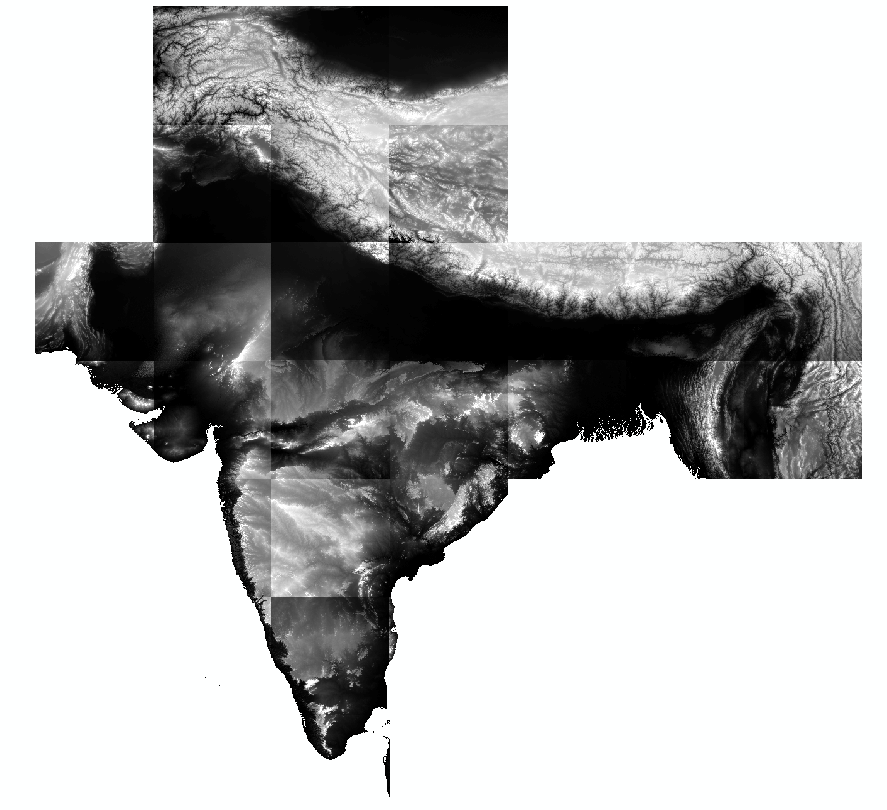
\includegraphics[width = 1\textwidth]{Figures/DEMTiles.png}
\caption{27 STRM digital elevation model (DEM) tiles are used for watershed delineation.}
\label{fig:demTiles}
\end{figure}

We perform following operation to delineate the catchment (a working code presented in the Listening \ref{lst:catDel}):
\begin{itemize}
\item{Remove sink and holes in DEM}
\item{Calculate flow direction raster}
\item{Calculate flow accumulation raster}
\item{Project pour point and using a buffer zone around to identify highest flow accumulation point}
\item{Calculate upslope-area raster}
\item{Convert upslope-area raster to shape files and calculate catchment area}
\end{itemize}

We format the names of delineation catchments, discharge data files, and water quality data files the same. We remove underscore and standardize the catchment names i.e. A. K$\textunderscore$Bridge $\rightarrow$ AKBridge. All the information is kept in the dataset sheet \emph{PourPoint950}.

\subsection{Running \emph{arcpy} outside ArcGIS environment}
Python scripting is essential for repetitive works like delineating catchment for several pour points. We use \texttt{arcpy}, python library of ArcGIS to automate the catchment delineation process. We use \texttt{anaconda} python-2.x distribution, \texttt{anaconda} also incorporates \texttt{spyder}, a Matlab like python GUI, which we use to write the python scripts for catchment delineation and database manipulation.

\noindent System Requirement for Windows operating system.
\begin{itemize}
\item ArcGIS installation (We use v10.3)
\item \href{https://www.anaconda.com/distribution/}{Anaconda} 32-bit installer
\end{itemize}

Installation automatic add the variables into system path. Copy all files from your ArcGIS directory \texttt{C:\textbackslash Python27\textbackslash ArcGISx6410.1 \textbackslash Lib\textbackslash site-packages} to Anaconda site package directory i.g. \texttt{C:\textbackslash Anaconda\textbackslash Libs\textbackslash site-packages}. Go to Anadonda root folder i.g. \texttt{C:\textbackslash Anaconda} find the \texttt{python.exe} and \texttt{pythonw.exe} run one by one as administrator. Now you should be able to load \texttt{arcpy} in your python console. To check this go to spyder console and type \texttt{import arcpy}, if you didn't get any error message, you successfully embedded \texttt{arcpy} to anaconda python distribution.

If the above process doesn't work still you can run a python script (*.py) inside ArcMap python console. Go to : Geoprocessing $\rightarrow$ Python $\rightarrow$ (Right Click) load script.

\subsection{Catchment selection for database} \label{sec:catSel} %%%%%%%%%%%%%%%%%%
We delineate 950 catchments but we found a lot of them are overlapping. As we select a pour point in the downstream it will delineate a large upslope area and overlap the catchments delineated with the pour points situated on upstream of the same stream. We delineate the catchments with an accumulation threshold of 2000. WRIS does not provide shapefiles of catchment but gives the area of the catchment in the unit of $km^2$. We found that 126 out of 950 catchments do not have catchment area information from WRIS so we discard these catchments. To verify the accuracy of our delineated catchments first we compute the area bias with WRIS catchment and discard the catchment which has a bias more than $\pm$20\%. Furthermore, we visually inspect remaining catchments and we finalize 567 catchments. The catchment shapefiles have a field \emph{area} denotes the area of the catchment in $km^2$. The projection of catchment in geographic coordinate system with the datum WGS1984: \texttt{+proj=longlat +datum=WGS84 +no\_defs +ellps=WGS84 +towgs84=0,0,0}. The range of catchment in the dataset varies from 40.67 to 804015.10 $km^2$. Outline of catchments are shown in Figure \ref{fig:histCat}, the gradient in the figure blue to red shows the increasing catchment area. The gauge station location of the catchment are shown with the colored circle, A histogram in the figures shows the area range of catchment in the database.

\begin{figure}[!h]
\centering
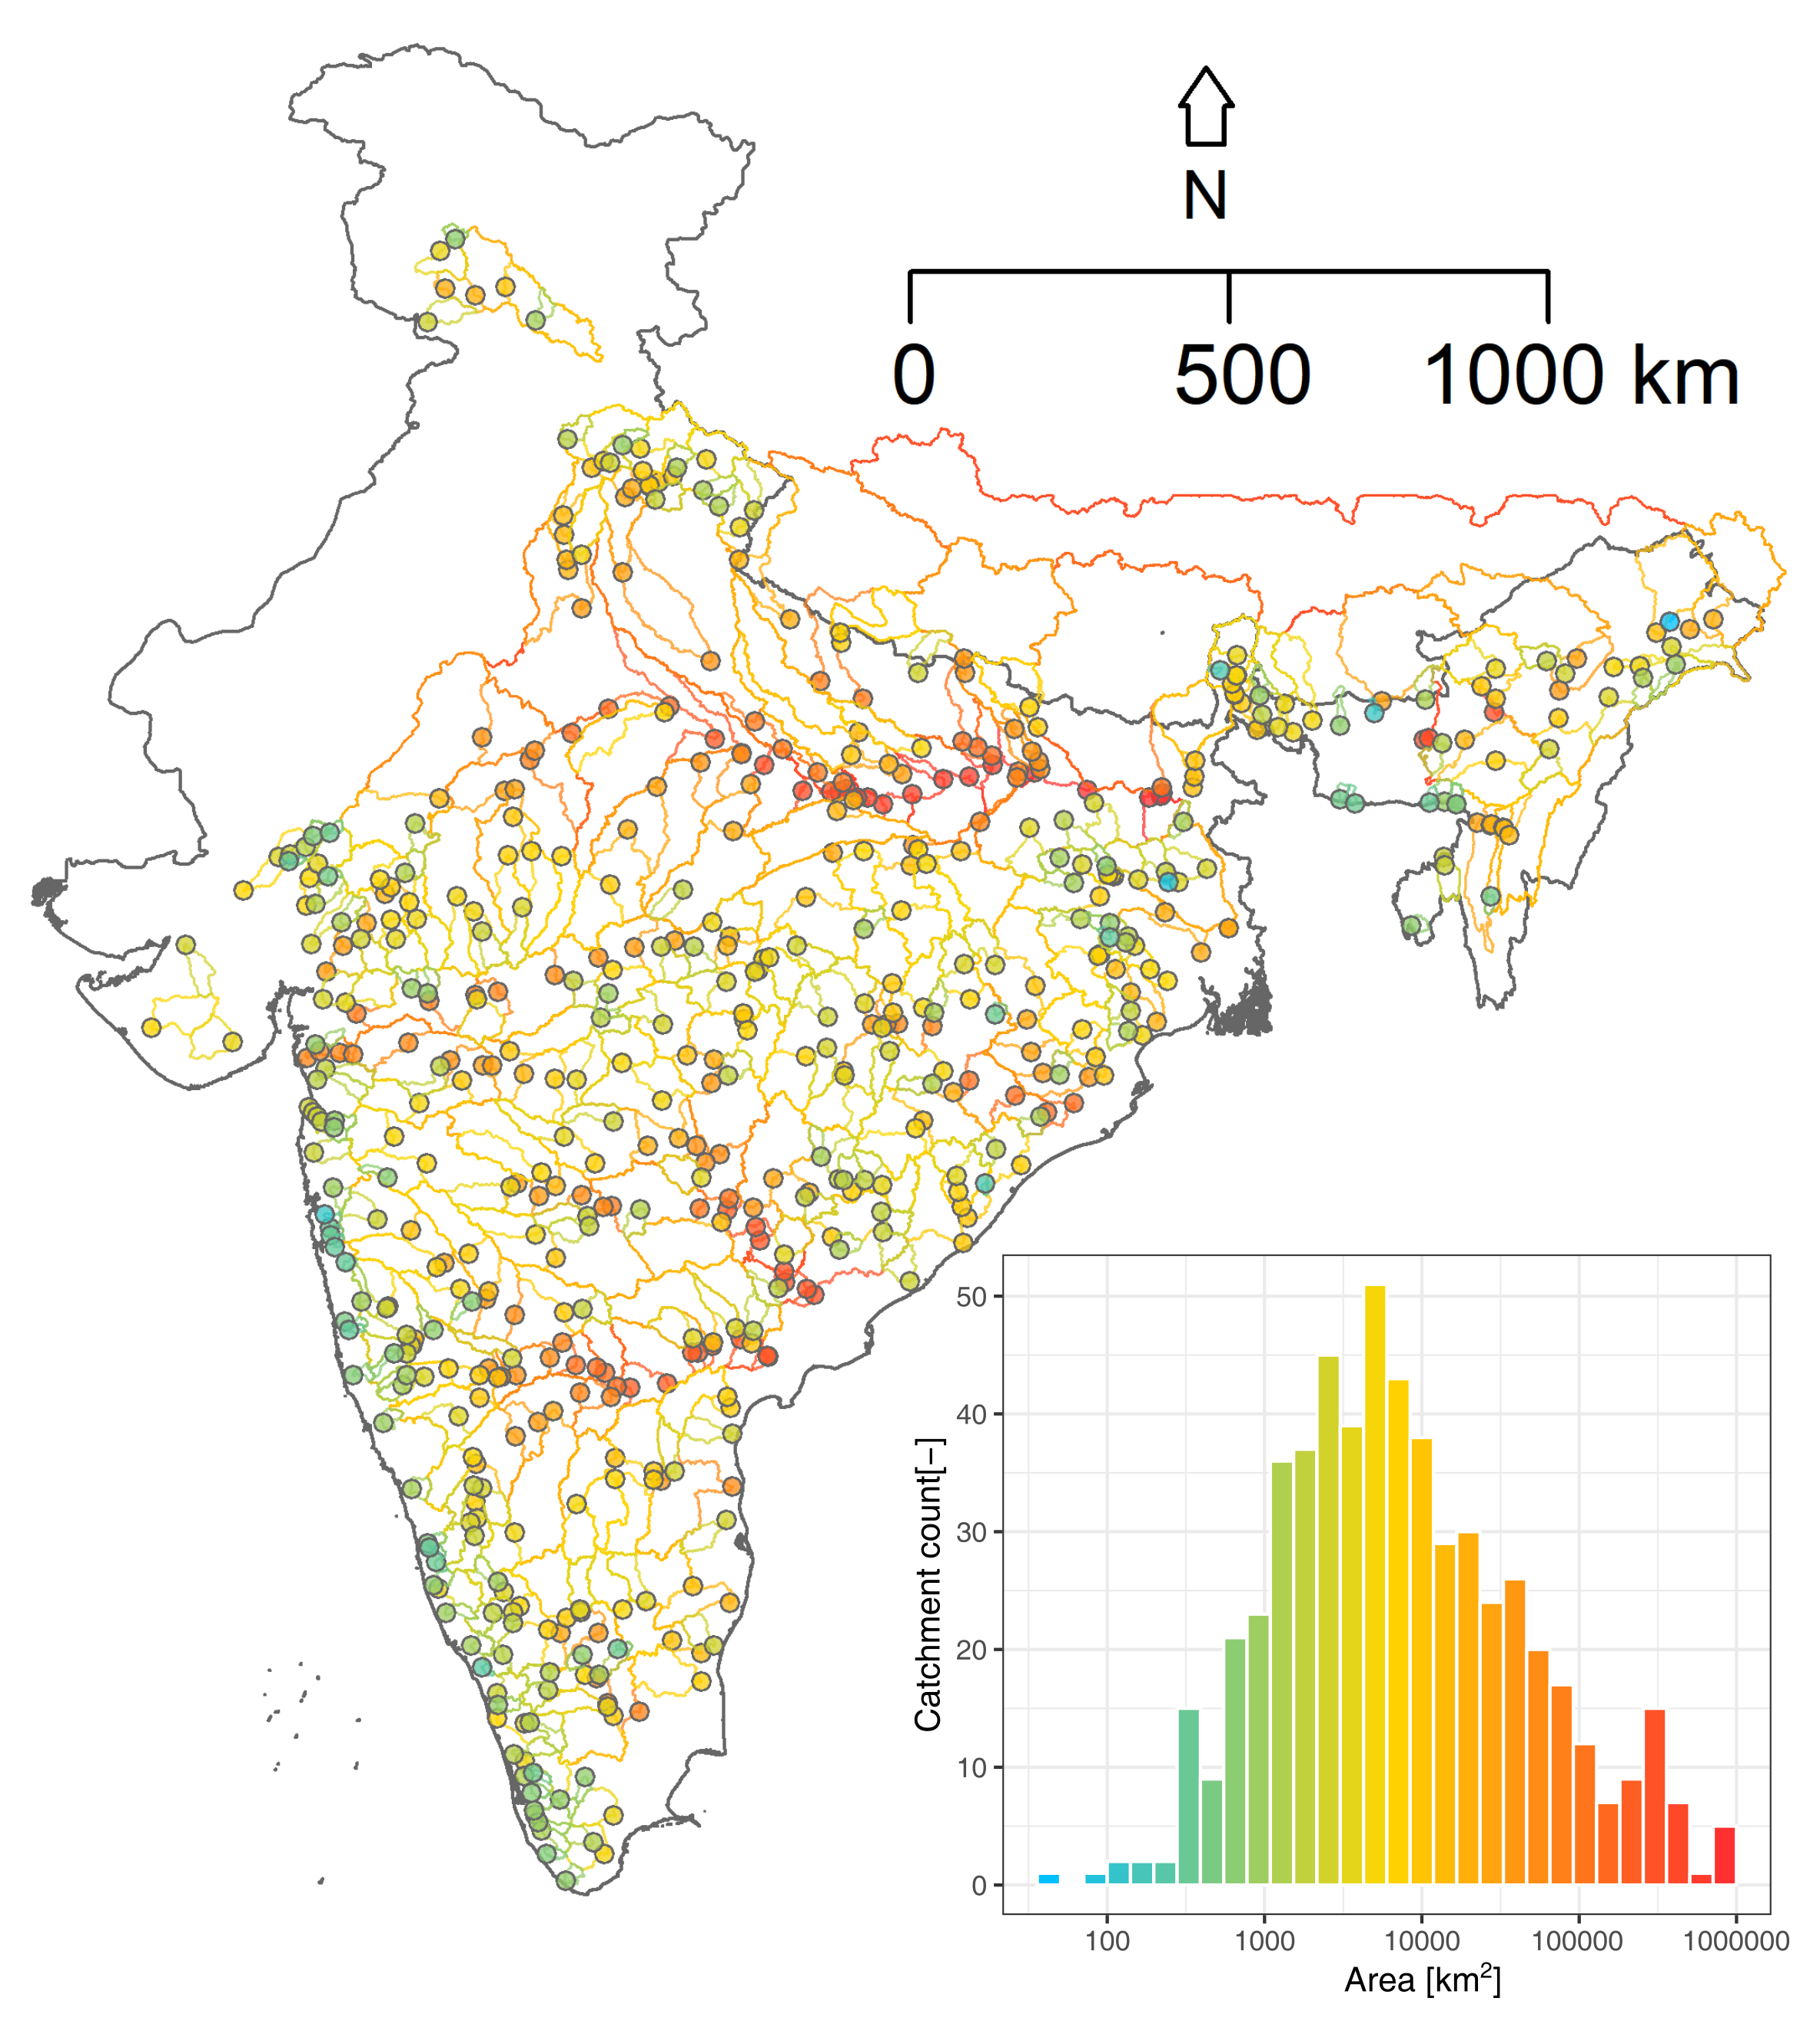
\includegraphics[width = 1\textwidth]{Figures/GaugeStation.png}
\caption{Boundaries for selected catchment are show in the figure. Each circle represents the pour point of a catchment. Colors of pour point and corresponding catchment boundary are same. Histogram represents the area's of catchments.  The color gradient sky blue to red represent increasing area of catchments.}
\label{fig:histCat}
\end{figure}

\clearpage
\section{Physio-climatic dataset} %%%%%%%%%%%%%%%%%%%%%%%%%%%%%%%%%%%%%%%%%%%%%% 
Mainly this document deals with the physio-climatic dataset, but we also collected the streamflow datasets for 412 catchments and water quality dataset for 366 gauge stations. The physio-climatic dataset divided into 7 categories named climate, geology, hydrology, land cover, land use, socioeconomic and topography. The climate category subdivided into 3 categories i.e. precipitation, temperature, and Evapotranspiration.

\subsection{Climate}
To develop climatic characteristics we purchase daily precipitation and temperature data from IMD Pune. The gridded precipitation data has a spatial resolution of 0.25 degree $\times$ 0.25 degree and the data available for January 01, 1901 to 31 December 31, 2015. The temperature dataset has a resolution of 1 degree $\times$ 1 degree.  It is much courser dataset then the precipitation data. We have 63 years of temperature data dated form January 01, 1951 to December 31, 2013. In the procession stage, we use a common temporal resolution of both the data(precipitation and temperature) which is January 01, 1951 to December 31, 2013. The unit of precipitation and temperature data is mm/day and $^\circ$C respectively.
\subsubsection{Precipitation}
IMD Pune provides the precipitation data in plain text format. Each file contains one year of daily data stacked by the days. Rows and columns denote latitude and longitude respectively. Our approach is to get the slice of each day and convert into a raster layer. Then using the shape a shapefile of each watershed we can crop the overlapped precipitation grid for that day. Rasterize daily precipitation layer with shapefile overlapped data for one catchment is shown in Figure \ref{fig:precipExt}. Then we use a weighted average of cropped pixels to get the mean daily precipitation for that catchment.

\begin{figure}[!h]
\centering
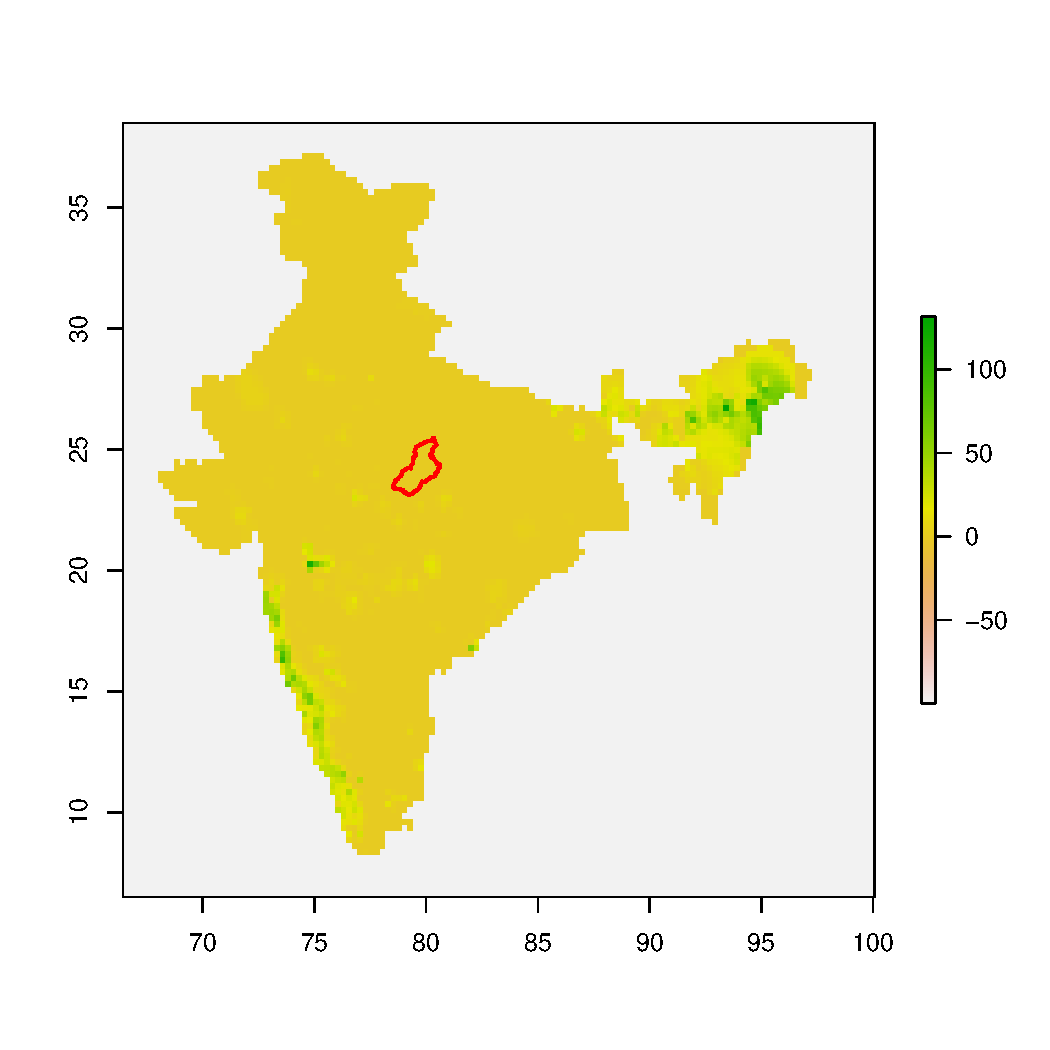
\includegraphics[width = 1\textwidth]{Figures/PrecipitationExt.pdf}
\caption{Daily precipitation layer rasterize then shapefile is overlapped to extract the values of precipitation}
\label{fig:precipExt}
\end{figure}

The process for precipitation data downscaling is shown in the Listening \ref{lst:precipDaily}. Later we use the Listening \ref{lst:precipMonthly} to convert monthly mean data for daily data. After that we computed several climatic characteristics form daily and monthly precipitation time series in with following code (Listening \ref{lst:precipChar}.

\subsubsection{Temperature}
The temperature data provided by IMD Pune has grid and ASCII text files for the period of 1951- 2013. The data has daily maximum, daily minimum and daily mean attributes in $^\circ$C. We follow a similar approach as precipitation data to extract mean daily data for a catchment. The steps taken to obtain daily temperature are shown in Listening \ref{lst:tempDaily}, see Figure \ref{fig:tempExt} to understand the temperature extraction method. After that we convert the daily to monthly temperature and steps required are shown in the Listening \ref{lst:tempMonthly}. 

\begin{figure}[!h]
\centering
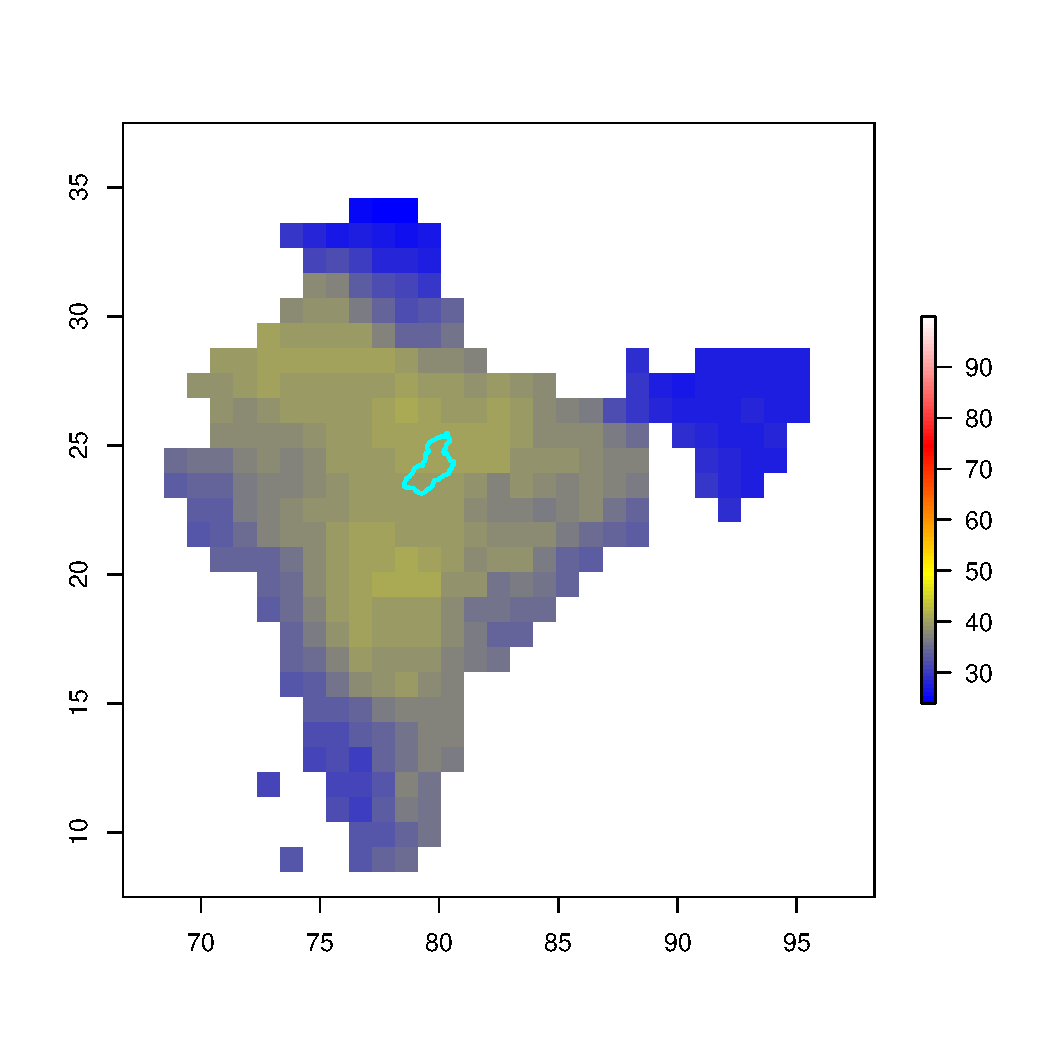
\includegraphics[width = 1\textwidth]{Figures/TemperatureExt.pdf}
\caption{Rasterised temperature overlapped with shapefiles to extract the daily temperature.}
\label{fig:tempExt}
\end{figure}

We use daily and monthly average temperature to get climatic characteristics listed in the database sheet \emph{Index}. A few characteristics are evapotranspiration, which we also compute with daily temperature using Hamon and Hargreaves equation. Discussed in detailed in Section \ref{sec:evapoTrans}.

\subsubsection{Evapotranspiration}\label{sec:evapoTrans}
We generated daily evapotranspiration (unit mm/day) for catchments using Hamon and Hargreaves equations. The equation uses daily maximum, mean and minimum temperature as an input. It also uses the latitude of the centroid of the catchment to compute evapotranspiration. The following function we required to compute daily evapotranspiration. \textbf{a.} Leap year (Listening \ref{lst:leapYr}): to know a year is a leap year. \textbf{b.} Solar radiation (Listening \ref{lst:solRad}): to calculate solar radiation based on Julian data and latitude of the centroid of the catchment. \textbf{c.} Hamon (Listening \ref{lst:hamon}): to compute daily evapotranspiration with Hamon equation. \textbf{d.} Hargreaves (Listening \ref{lst:harg}): to compute daily evapotranspiration with Hargreaves equation. 

\subsection{Geology}
Geology is the study of earth's surface and the consisting material. To understand the formation of earth's surface we use Global Lithological Map (GLiM) database \citep{hartmann2012new}. Lithology shows us the geochemical, mineralogical, and physical characteristics of rocks. This dataset consists of surface and subsurface lithological formation of earth in 16 categories. The categories are shown in the database documentation Index sheet. We extract \% cover each geological formation with a weighted average of specific categories for each catchment. The steps taken are shown in the Listening \ref{lst:geology}

\subsection{Hydrology}
Catchments' hydrologic characteristics consist of stream density, stream orders, etc. To compute hydrologic characteristics, we need a DEM with a projected coordinate system, initially, it was a geographic coordinate system. We use the Universal Transverse Mercator coordinate system for projection because the cylindrical projection preserves Area and minimizes distortion of distance for small extent. We use 6- \href{http://spatialreference.org/ref/epsg/32642/}{UTM zones} (UTM-42N or EPSG:32642 to UTM-47N or EPSG:32647). The Figure \ref{fig:UTM} shows various UTM zones covers India. 

\begin{figure}[!h]
\noindent
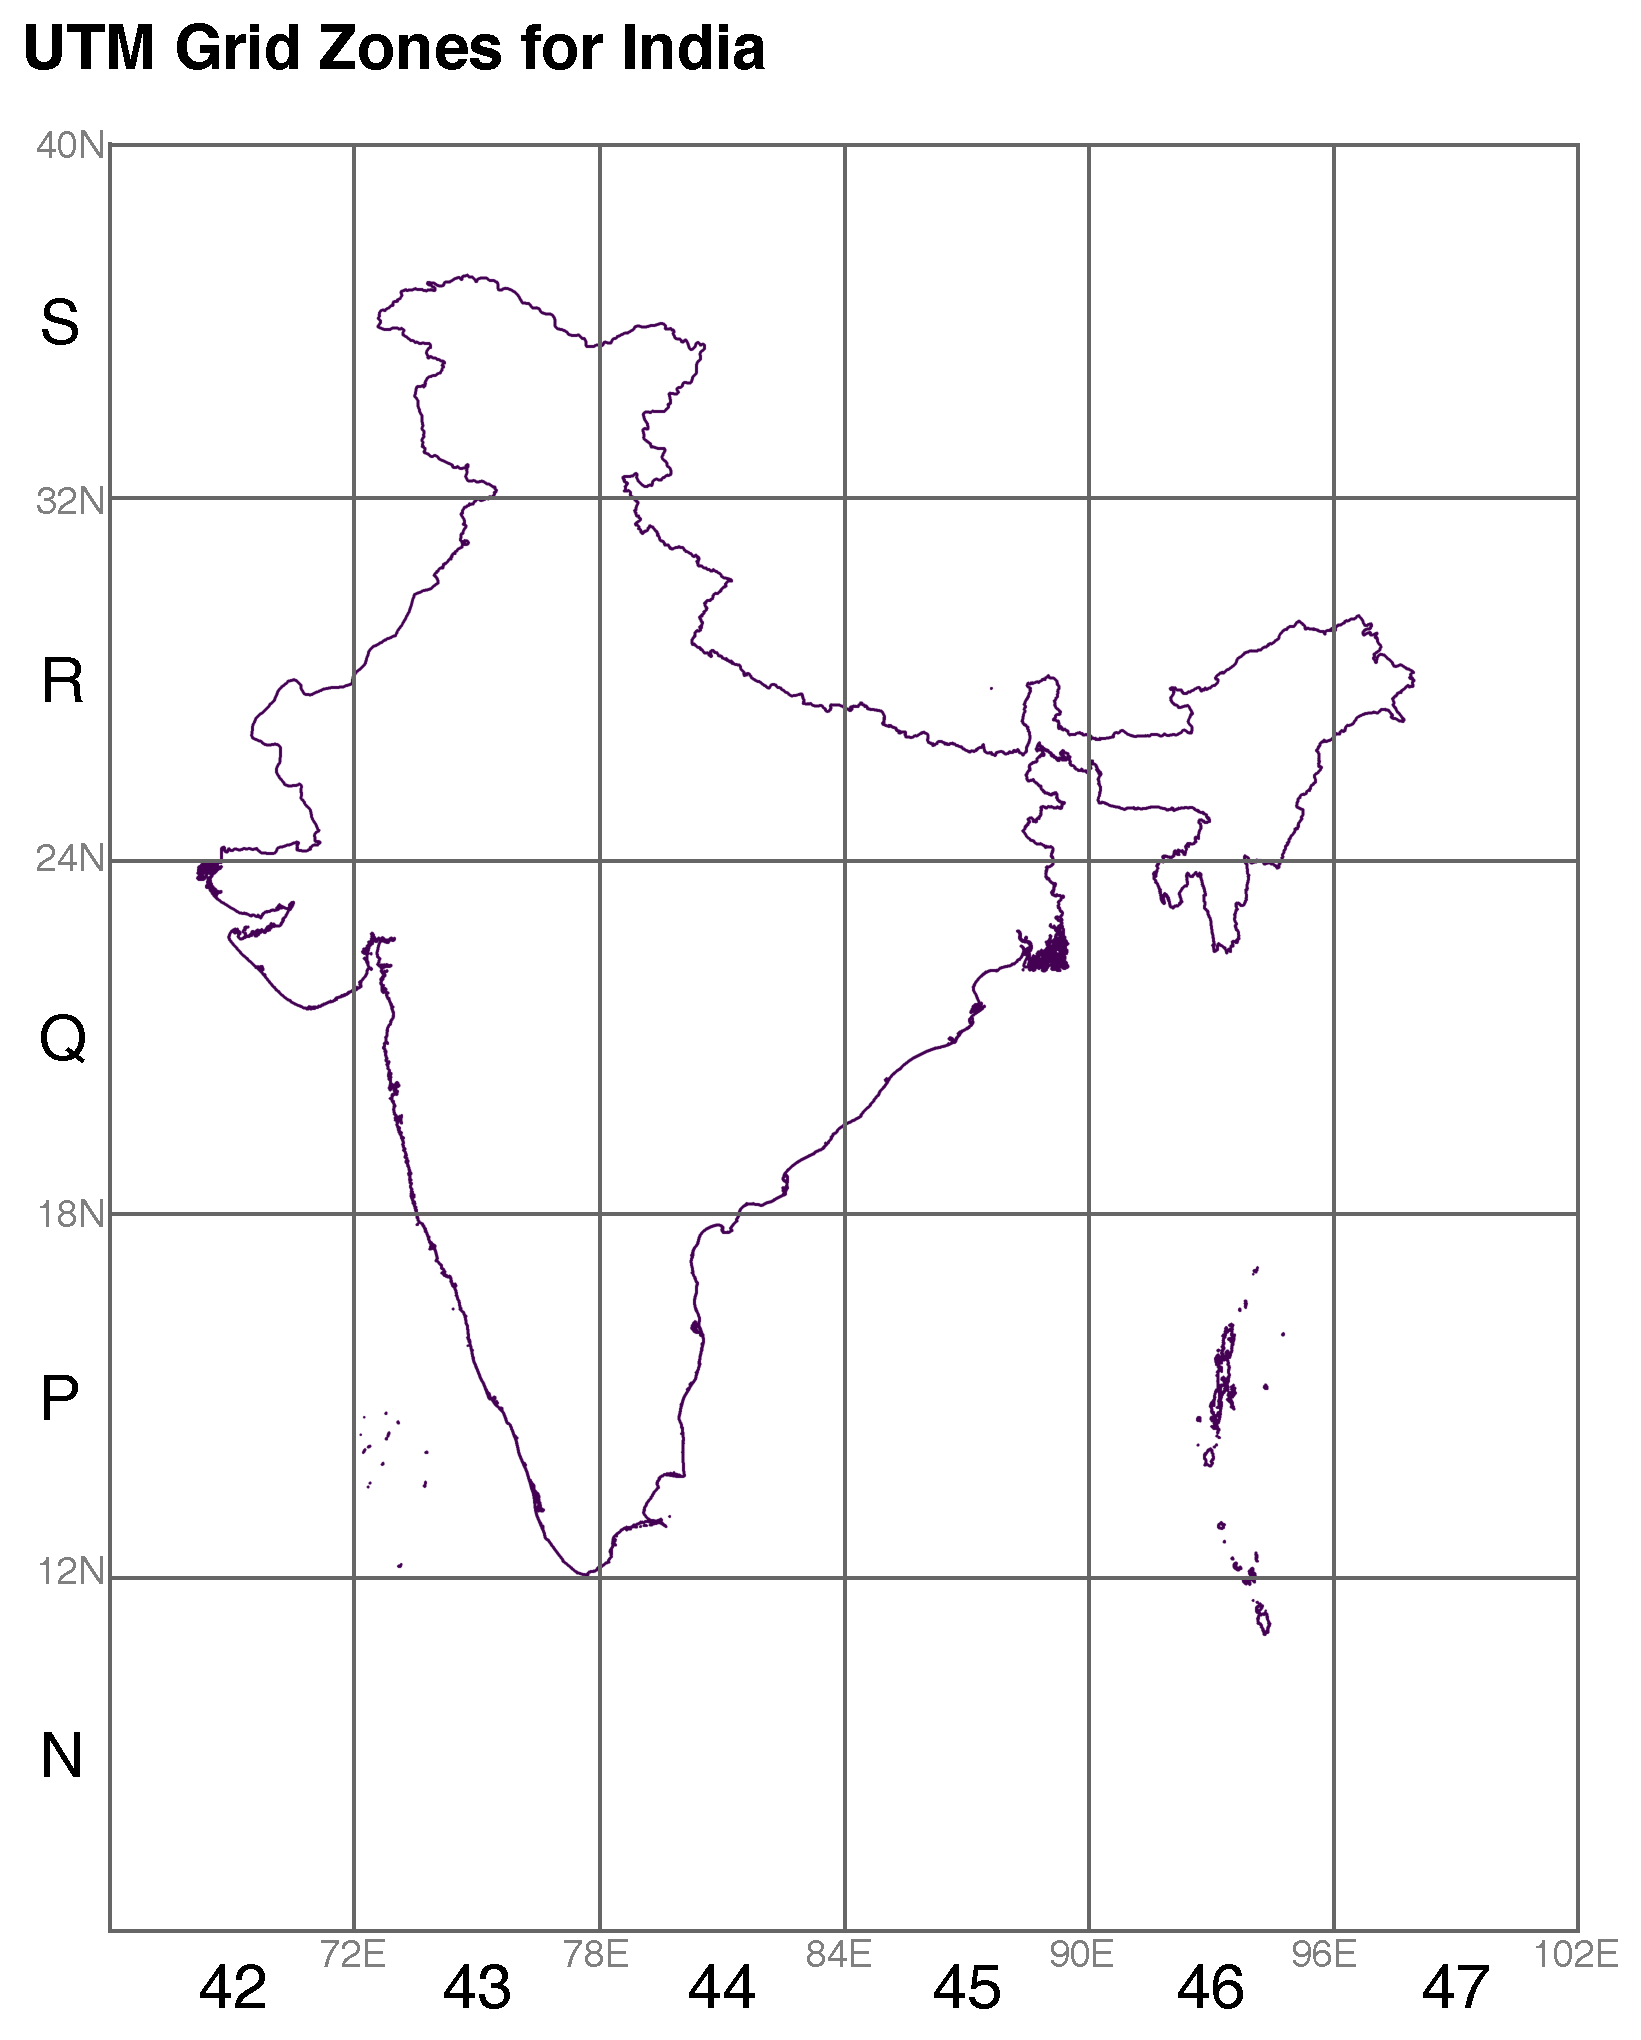
\includegraphics[width = 1\textwidth]{Figures/UTM_Zones.pdf}
\caption{UTM projection zones used for India}
\label{fig:UTM}
\end{figure}

We use \textbf{R} in most of our dataset development but we found generating streams from DEM are much easier using \href{https://grass.osgeo.org/}{GRASS} (Geographic Resources Analysis Support System). GRASS is an open-source Geographic Information System (GIS) software suite which is a powerful tool for geospatial data management, analysis and image procession. To make analysis reproducible and automated we use \href{https://cran.r-project.org/web/packages/rgrass7/index.html}{rgrass7} package which is an interpreted interface between \textbf{GRASS} and \textbf{R}.
We are explaining the process to run GRASS from R using rgrass7 package in the next Section \ref{sec:grass}.

\subsubsection{Setting-up GRASS}\label{sec:grass}
We process the DEM to compute hydrology characteristics with the following steps shown in the Listening \ref{lst:hydroProc}. Before running any GRASS module we need to set up the GRASS environment for R. First we need to download GRASS GIS setup. We use GRASS GIS v7.6. GRASS GIS is installed in the location of \texttt{C:/Program Files/GRASS GIS 7.6}. Then we need `rgrass7' package for R to initiate GRASS session. The following piece of code required to set up the GRASS session.

\begin{minipage}{1\linewidth}
\begin{verbatim}


# Initiate GRASS session 
if(.Platform$OS.type == "windows"){gisbase = "C:/GRASS GIS 7.6"}
initGRASS(gisBase = gisbase,
          home = tempfile(),
          override = TRUE)
\end{verbatim}
\end{minipage}

\subsubsection{Stream order processing}
With GRASS we perform the following step to get the stream and order shapefiles for each catchment.
\begin{enumerate}
\item Load the DEM to conditioning, which required remove sink and fill, using GRASS \texttt{r.hydrodem} module.
\item Then conditioned DEM used to compute flow accumulation raster in the module \texttt{r.watershed}
\item After that we use \texttt{r.stream.extract} to generate stream and direction raster.
\item The stream raster used in \texttt{r.stream.order} to develope stream order map.
\end{enumerate}

\begin{figure}
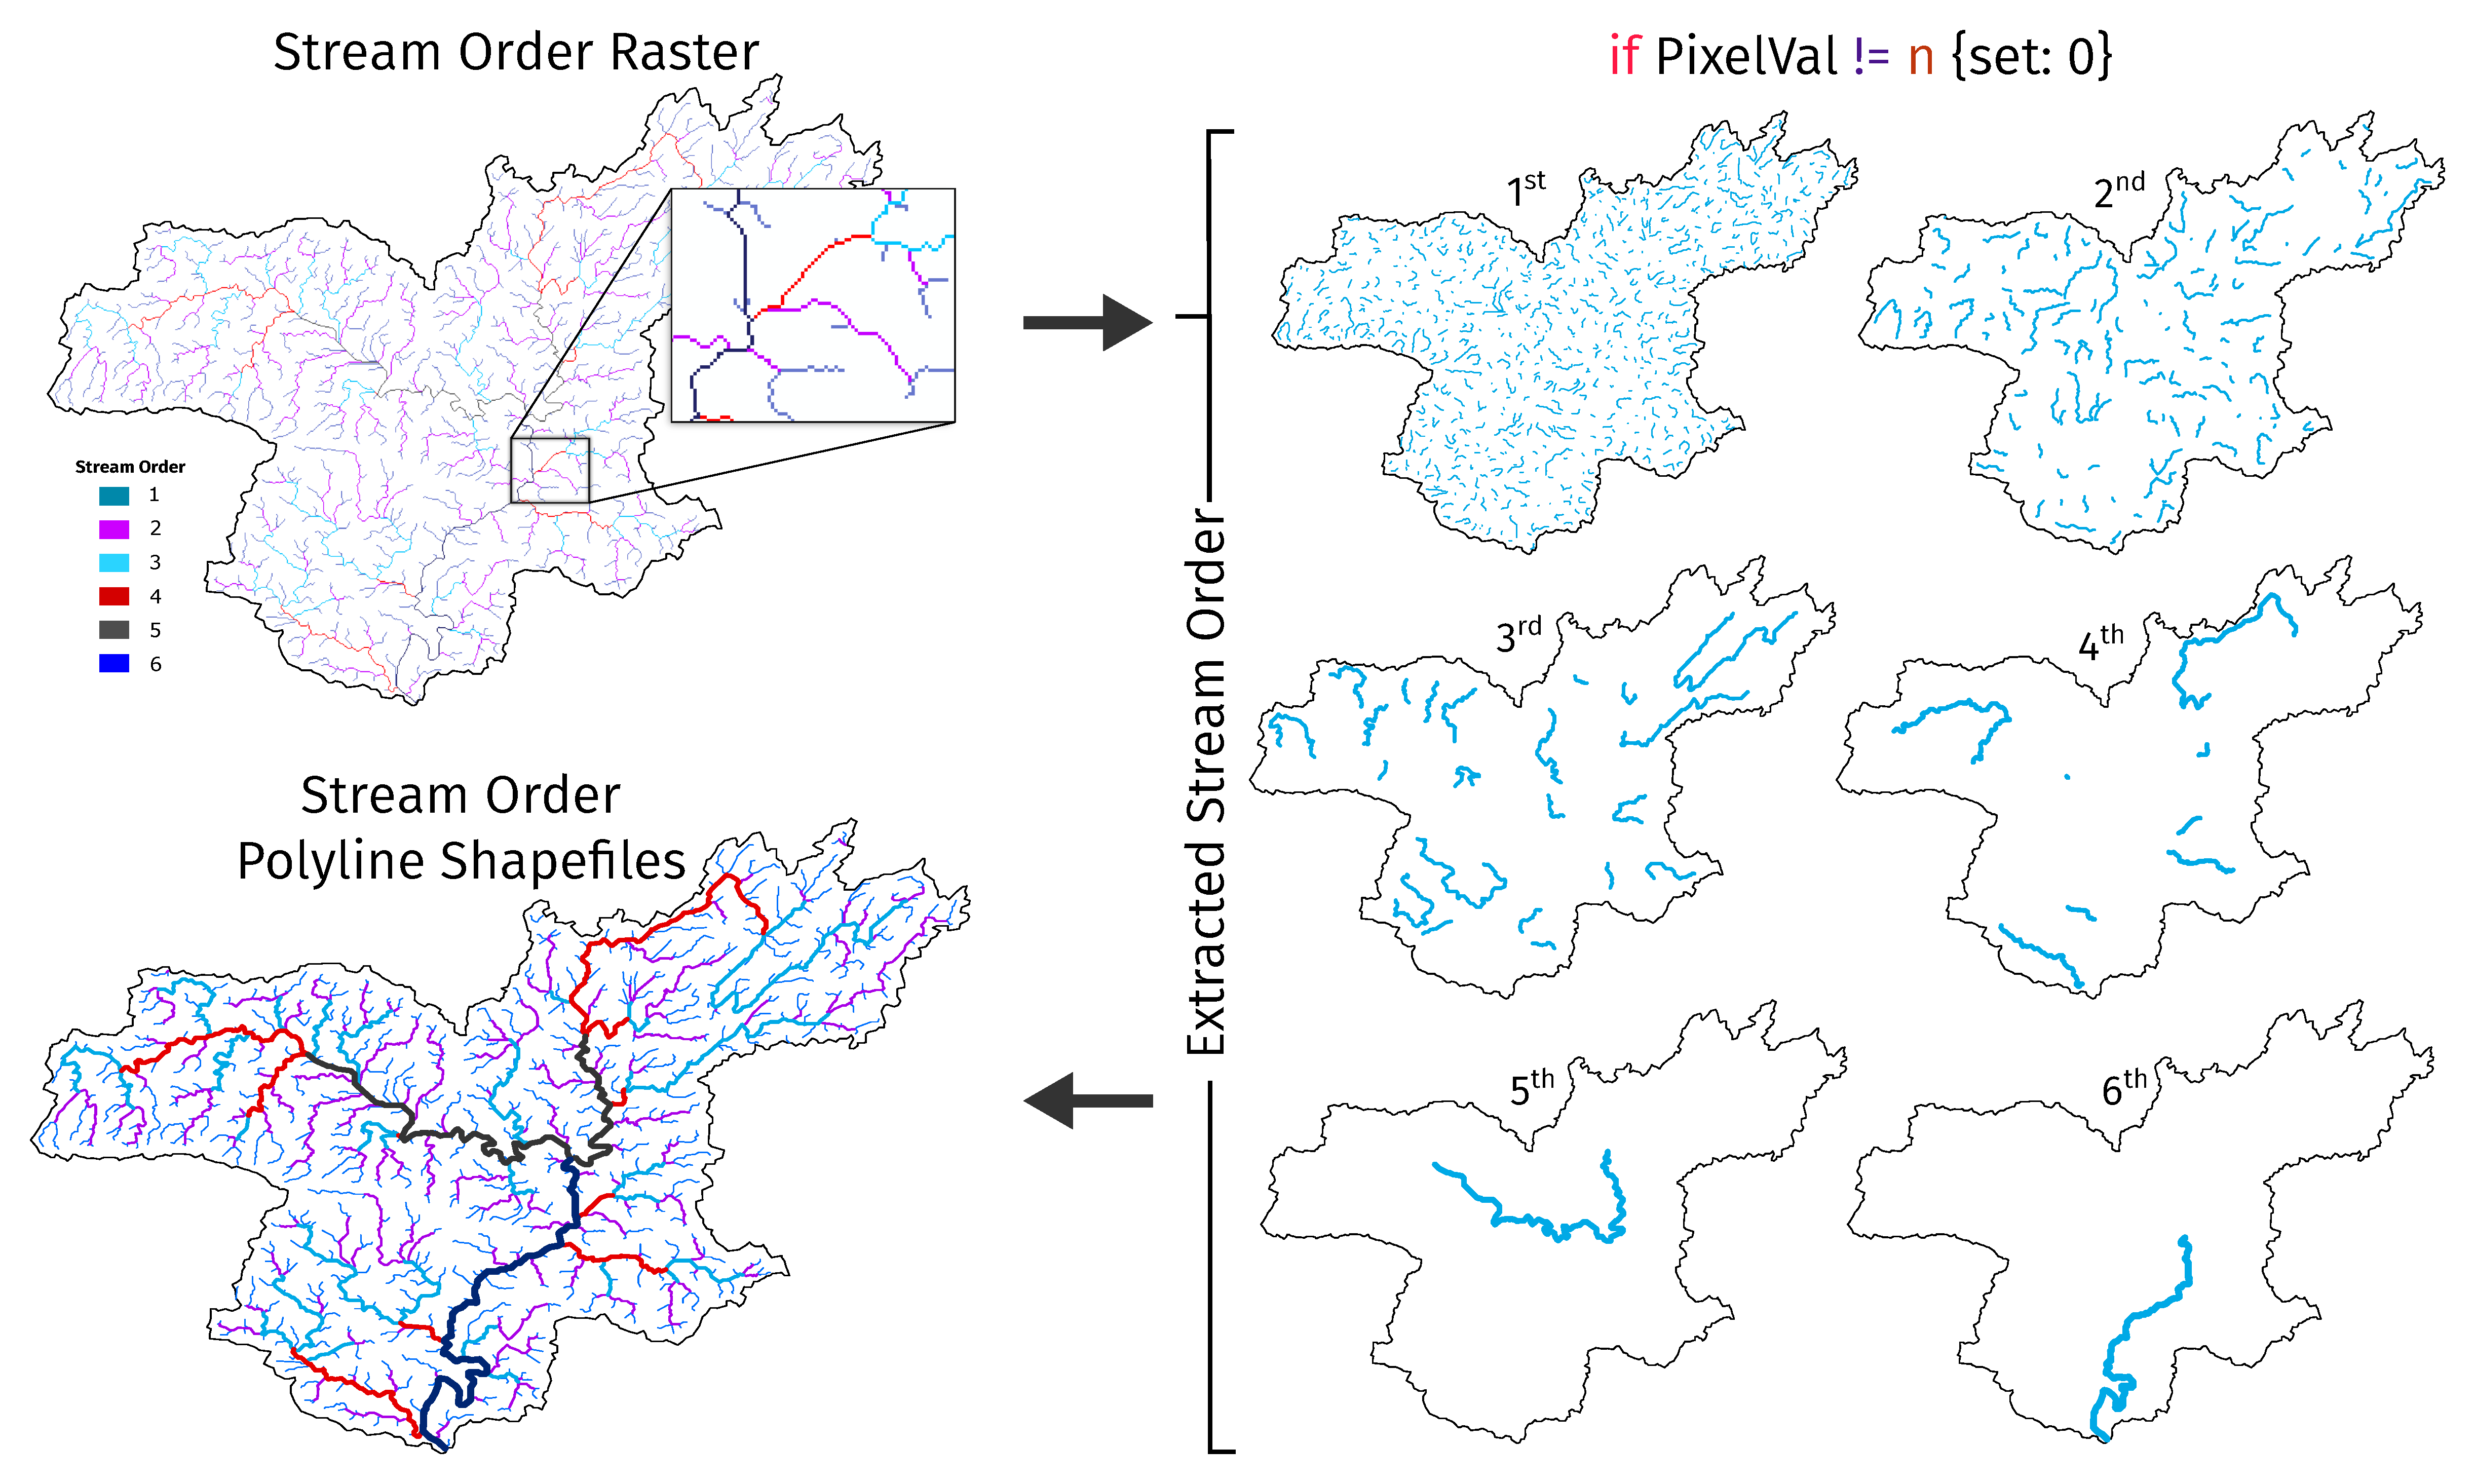
\includegraphics[width = 1\textwidth]{Figures/StreamOrderLength.pdf}
\caption{Extraction of stream order from raster.}
\label{fig:streamOrder}
\end{figure}

The working code is presented in the Listening \ref{lst:hydroProc}. After getting stream order we extract/compute hydrological characteristic using the process presented in the Listening \ref{lst:hydroExt}

\subsection{Land cover} 
We use the land cover map for south-east Asia from the year of 2000. The source of the dataset is \citet{stibig2003land}. The data is 1km resolution raster dataset. It contains 47 classes where each pixel can hold a value between 0 to 46. Some of the categories like tropical evergreen subtropical evergreen, temperate broad-leaved, tropical montane, tropical semi-evergreen, temperate conifer, etc.(see Figure \ref{fig:lc}). We clip land cover class data from raster using extract function form \textbf{R} and based on a weighted average on pixel we calculate the \% of land cover in covered by each category for each catchment.

\begin{figure}[!h]
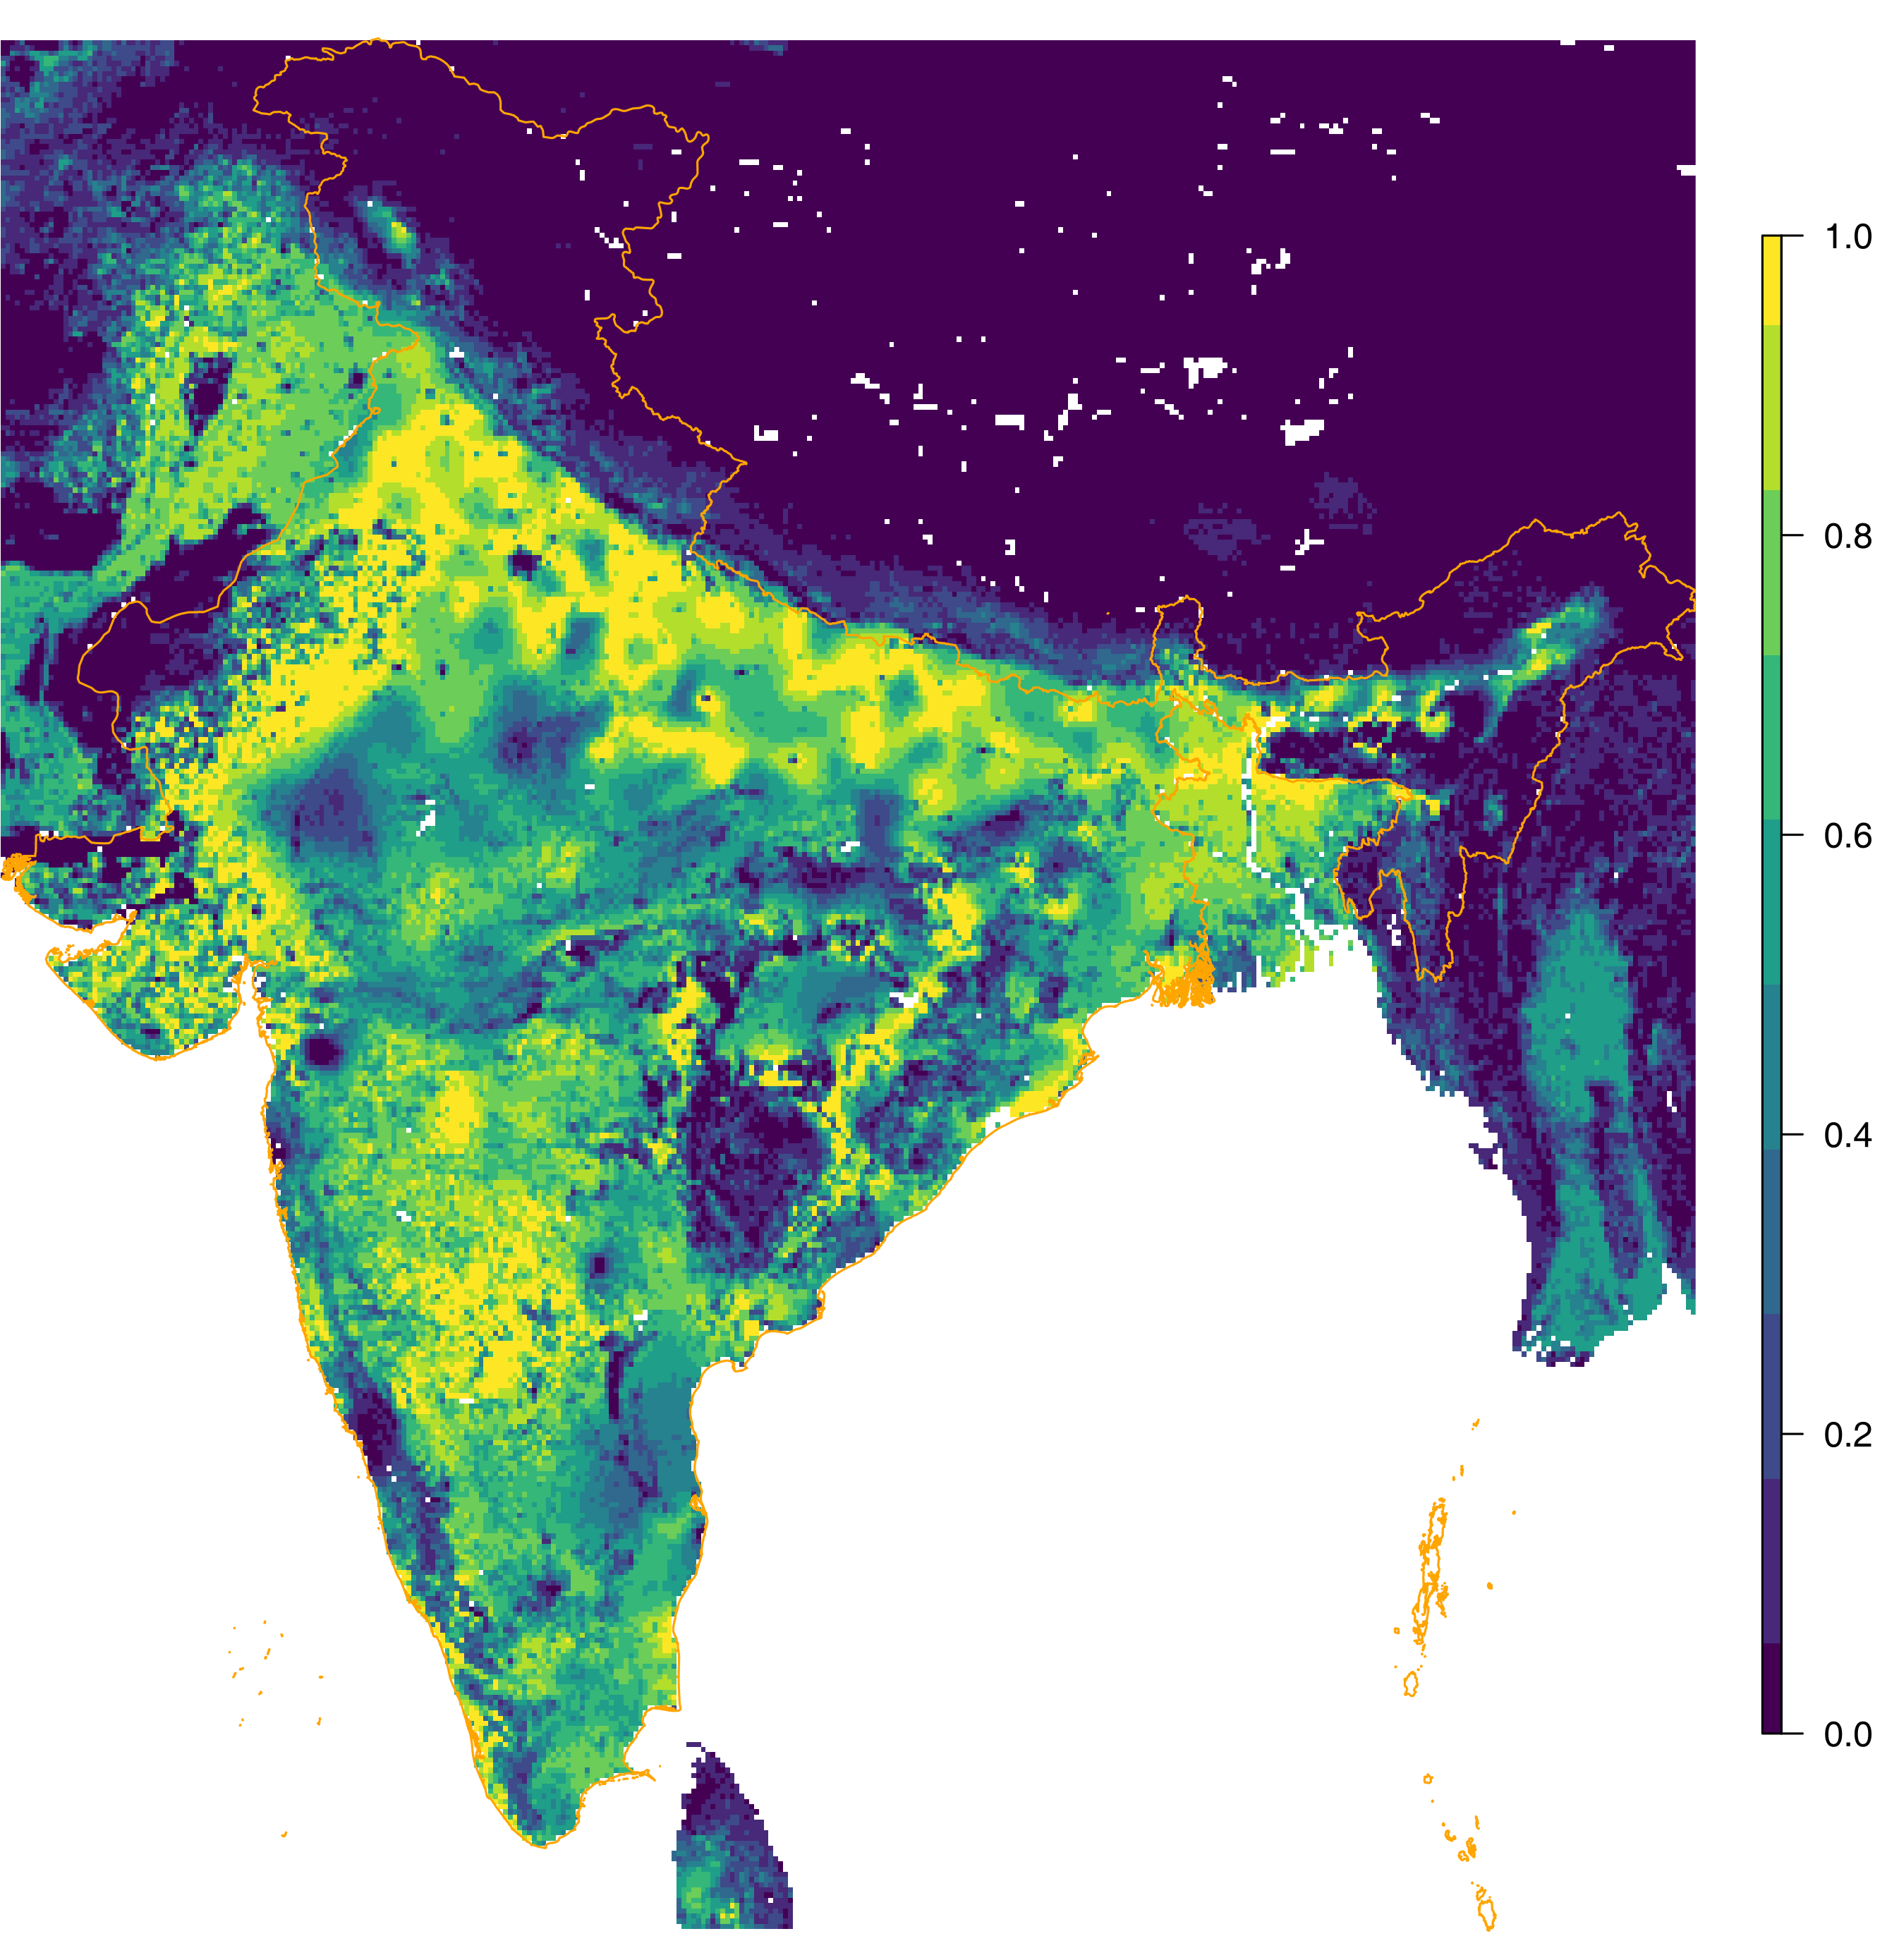
\includegraphics[width = 1\textwidth]{Figures/LC.png}
\caption{Dataset for land cover}
\label{fig:lc}
\end{figure}

The table of land cover categories are shown in the Table \ref{tab:lc}.
\begin{table}[!h] % using https://www.tablesgenerator.com/
\begin{tabular}{llll}
\hline
SN & Category                      & SN & Category                        \\ \hline
1  & Sea                           & 25 & Desert Grasslands               \\
2  & Tropical Evergreen            & 26 & Alpine Meadow                   \\
3  & Subtropical Evergreen         & 27 & Alpine Grasslands               \\
4  & Temperate Broadleaved         & 28 & Sparse vegetation (cold)        \\
5  & Tropical Montane              & 29 & Sparse vegetation (hot)         \\
6  & Tropical Semievergreen        & 30 & Gobi                            \\
7  & Temperate Conifer             & 31 & Desert (cold)                   \\
8  & Subtropical Conifer           & 32 & Thorn Scrub / Desert (hot)      \\
9  & Tropical Moist Deciduous      & 33 & Irrigated Intensive Agriculture \\
10 & Tropical Dry Deciduous        & 34 & Irrigated Agriculture           \\
11 & Junipers                      & 35 & Slope Agriculture               \\
12 & Mangroves                     & 36 & Rainfed Agriculture             \\
13 & Degraded Forest               & 37 & Current Jhum                    \\
14 & Dry Woodland                  & 38 & Swamp                           \\
15 & Thorn Forest/Scrub (Northern) & 39 & Coral reef                      \\
16 & Thorn Forest/Scrub (Southern) & 40 & Water Bodies                    \\
17 & Shrubs                        & 41 & Snow                            \\
18 & Abandoned Jhum                & 42 & Barren                          \\
19 & Sparse woods                  & 43 & Bare Rock                       \\
20 & Bush                          & 44 & Salt Pans                       \\
21 & Coastal vegetation            & 45 & Mud Flats                       \\
22 & Savannah                      & 46 & Settlement                      \\
23 & Plain Grasslands              & 47 & No Data                         \\
24 & Slope Grasslands              & 48 & Cropland field                  \\ \hline
\end{tabular}
\caption{The land cover categories exists in the dataset.}
\label{tbl:lc}
\end{table}

We add CROP\_LAND field in the dataset from Global Croplands in 2000 map. It shows the proportion of each 5 minutes (10km) grid cell land area that is under cropland \citep{ramankutty2010global}. We use a similar data extraction technique as land cover to get the mean cropland cover for each catchment.

\subsection{Land use}
To develop the land use dataset we use the anthropogenic biome of the world map for the year 2000. The map has 19 categories. Provided data is in raster grid (GeoTIFF) format and each pixel has a value that is associated with a land use category. The land use category is shown below in Table \ref{tab:lu}. 

\begin{table}[!h]
\begin{tabular}{llllll}
\hline
SN & Pixel & Category                        & SN & Pixel & Category                            \\ \hline
1  & 11    & Urban                           & 11 & 41    & Residential rangelands              \\
2  & 12    & Mixed settlements               & 12 & 42    & Populated rangelands                \\
3  & 21    & Rice villages                   & 13 & 43    & Remote rangelands                   \\
4  & 22    & Irrigated villages              & 14 & 51    & Residential woodlands               \\
5  & 23    & Rainfed villages                & 15 & 52    & Populated woodlands                 \\
6  & 24    & Pastoral villages               & 16 & 53    & Remote woodlands                    \\
7  & 31    & Residential irrigated croplands & 17 & 54    & Inhabited treeless and barren lands \\
8  & 32    & Residential rainfed croplands   & 18 & 61    & Wild woodlands                      \\
9  & 33    & Populated croplands             & 19 & 62    & Wild treeless and barren lands      \\
10 & 34    & Remote croplands                &    &       &                                     \\ \hline
\end{tabular}
\caption{Land use categories and the corresponding pixel values in the dataset.}
\label{tab:lu}
\end{table}

\begin{figure}[!h]
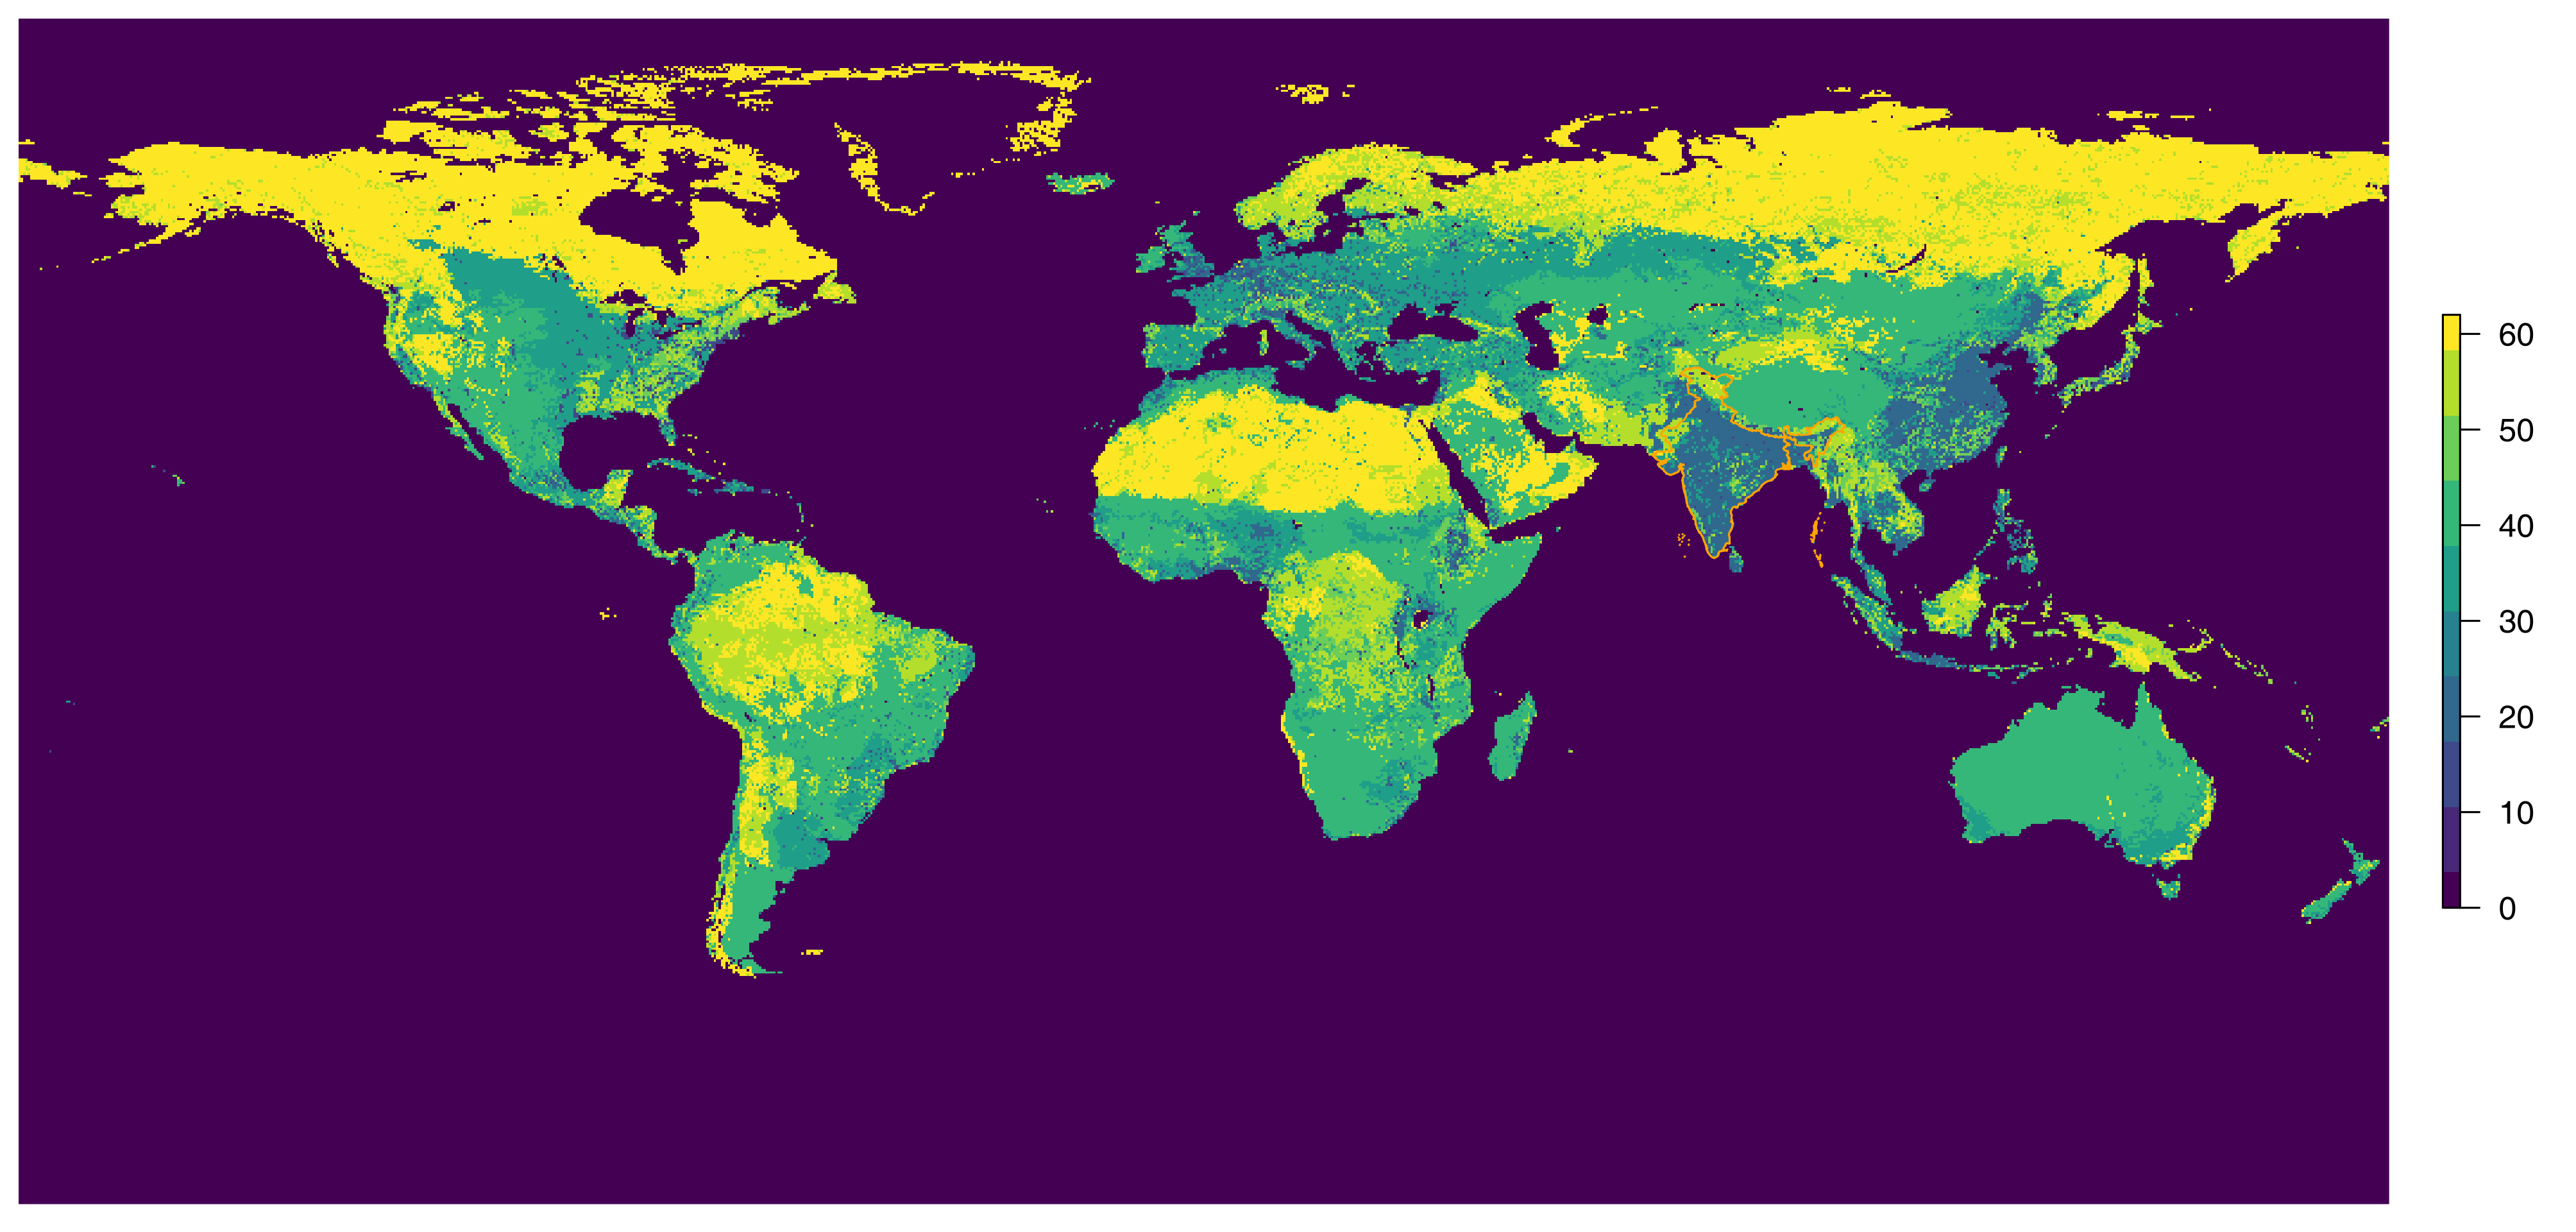
\includegraphics[width = 1\textwidth]{Figures/LU.png}
\caption{Dataset for land use}
\end{figure}

\subsection{Socioeconomic}
The socioeconomic dataset is the collection of characteristics represents human influence in the catchment. As socioeconomics is the study of how economic activity affects the social process, we use a socioeconomic dataset to quantify the anthropogenic effect on the catchment. The socioeconomic data set consists of a characteristic such as population density, human footprint index, suitability for agriculture, total nitrogen consumption, total nitrogen consumption, total nitrogen consumption, gross domestic production per capita (purchasing power parity), and human development index. The detail discretion and citation can be found in the database documentation. In the future, we will add other classes of socioeconomic data.

All the data is available in the raster grid format, we process it by cropping the raster with shapefile and the compute weight age average for each pixel to get mean characteristic values for each catchment.  

\subsection{Soil} 
We acquire soil characteristics from SoilGrids1km — Global Soil Information Based on Automated Mapping. Soil grid data is available in 6 layers (0-5cm, 5-15cm, 15-30cm, 30-60cm, 60-100cm, 100-200cm) and it consists soil, organic carbon (g kg$^{-1}$), soil pH, sand, silt and clay fractions (\%), bulk density (kg m$^{−3}$), cation-exchange capacity (cmol+/kg), coarse fragments (\%), soil organic carbon stock (t ha$^{−1}$). \citet{hengl2014soilgrids1km} develop the dataset and can be obtained freely from \href{https://soilgrids.org/}{Soilgrid}. We also gather permeability and porosity data form GLobal HYdrogeology MaPS (GLHYMPS) of permeability and porosity \citep{gleeson2014glimpse}

\subsubsection{Soil fractions} 
We extract soil fraction and chemical characteristics form SoilGrids1km dataset. We use layers of the mean depth of available soil products such as for soil organic carbon we use a layer of soil at 2.5 cm (mean of 0 to 5cm). The dataset provided in the raster grid. We extract with mean values of characteristics with weighted pixel values covered by catchment shapefiles. 
\subsubsection{Porosity and Permeability}
We extract porosity and permeability of the soil, from \citet{gleeson2014glimpse}. It is a global porosity and permeability database available in spatial polygons shapefiles. Each polygon has properties fields of porosity, permeability without permafrost, permeability with permafrost. We consider permeability without permafrost as permeability for our database. We rasterize the polygon layer (shapefiles) with field with porosity and permeability into 2 separate raster gird. Then we crop and extract mean values or characteristics for each catchment. We are demonstrating the polygon layer into Figure \ref{fig:PorPer}.
 
\begin{figure}[!h]
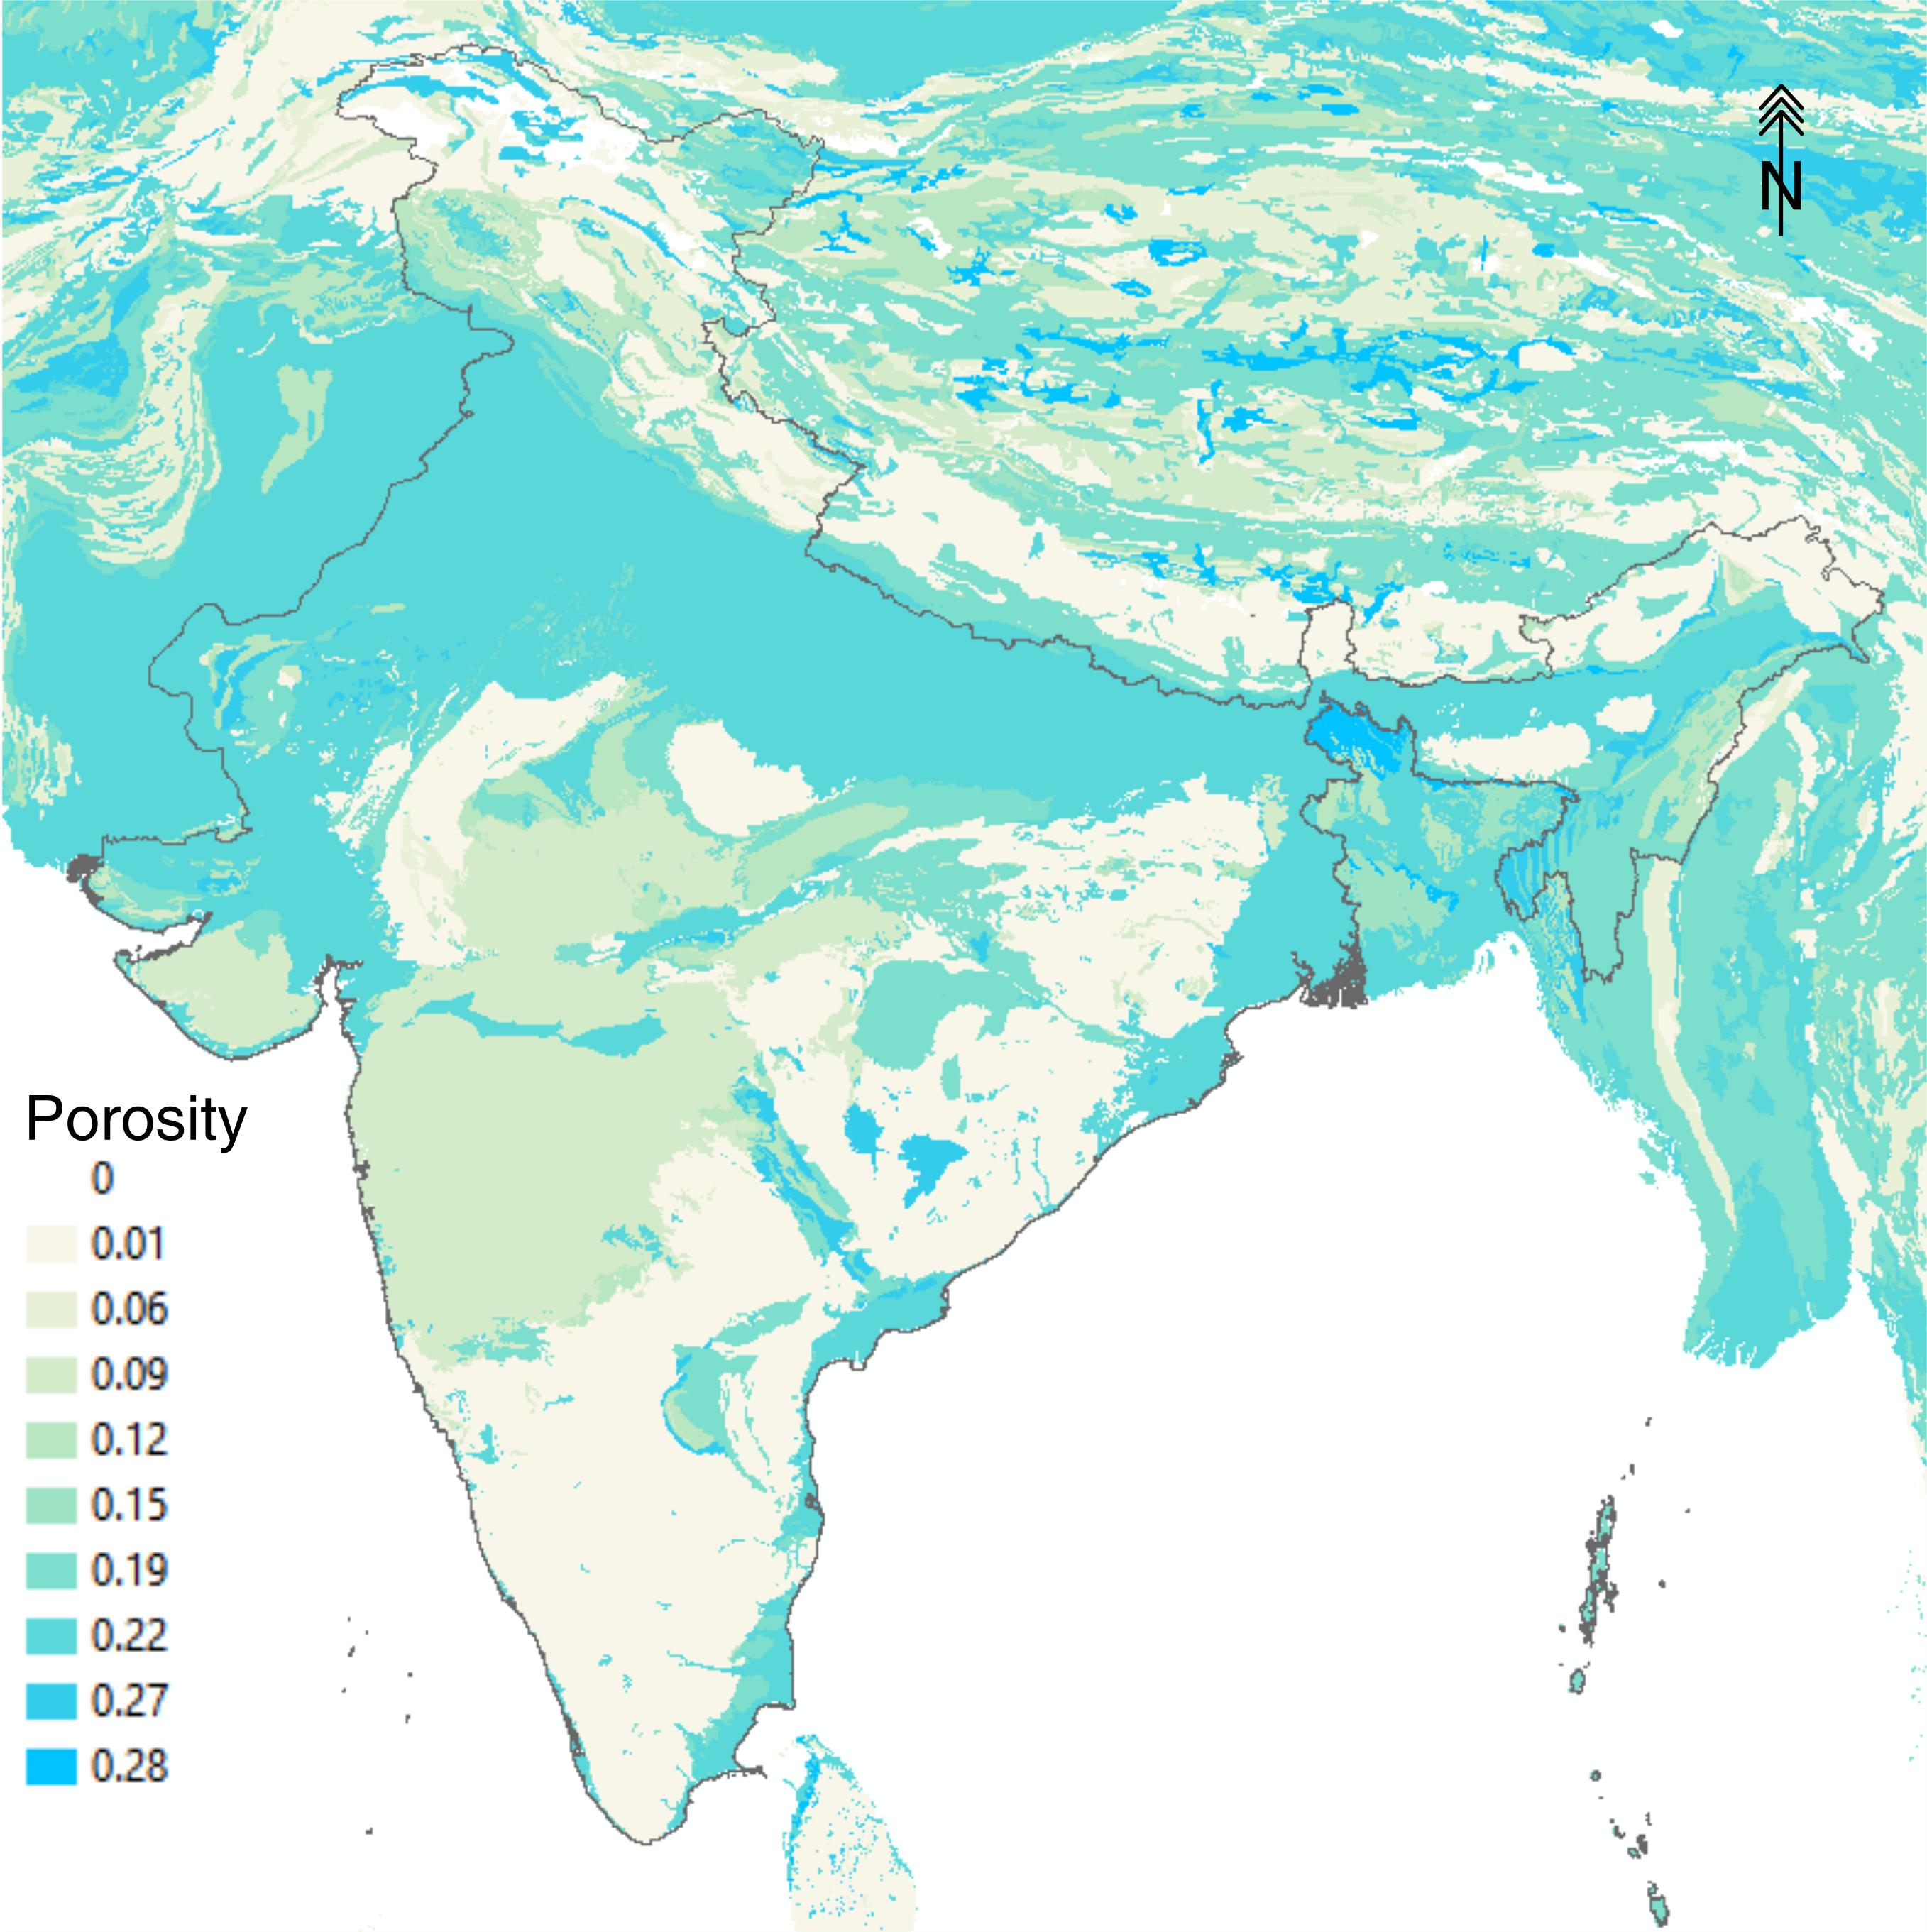
\includegraphics[width = 1\textwidth]{Figures/PorPer.png}
\caption{Porosity map for India}
\label{fig:PorPer}
\end{figure}

\subsection{Topography} 
To understand the physical features of our catchment we compute various topographical characteristics such as mean watershed elevation, mean watershed aspect, aspect-northness, relief ratio, tangential curvature, mean watershed slope, etc. A full list of topographical characteristics is available in the database. Most of the characteristics are derived from DEM. STRM DEM layers are obtained from the Consultative Group for International Agricultural Research \href{http://srtm.csi.cgiar.org/SELECTION/inputCoord.asp}{(CGIAR)}. The steps to compute topographical characteristics are presented in the Listening \ref{lst:topoExt}. 

The topographic wetness index is commonly used to quantify topographic control on hydrological processes. It is defined as: $\ln{\frac{a}{tan(b)}}$. where ${\displaystyle a}$ a is the local upslope area draining through a certain point per unit contour length and ${\displaystyle \tan (b)}$ is the local slope in radians. \textbf{R} does not have any module to compute the Topographical wetness index(TWI). So we use GRASS with rgrass7 package to get the TWI map for each catchment. One crucial step to project DEM map into UTM otherwise GRASS yields negative TWI. The computation of the TWI map is shown in the listening \ref{lst:hydroProc}. A sample map for TWI is also presented in Figure \ref{fig:twi}

\begin{figure}[!h]
\centering
\includegraphics[width = 1\textwidth]{Figures/TWI.png}
\caption{Topographic index for a catchment.}
\label{fig:twi}
\end{figure}

\clearpage
\section{Other datasets}
\subsection{Discharge dataset}\label{sec:dd} %%%%%%%%%%%%%%%%%%%%%%%%%%%%%%%%%%%%%%%%%%%%%%%%%%%%
We obtain discharge data from WRIS India for 412 catchments. We do not have any gauge discharge data for Ganga, Indus, and Brahmaputra river basins. Discharge data provided in the daily time stamp but data availability vary for each gauge station. The data has the following columns 1. Day: Date of the observation, 2. Data Type: shows the measurement with respect to absolute gauge(HZS) or mean sea level(HHS), 3. Mean Gauge: gauge height in meter, 4. Discharge: runoff measured in cubic meter/sec (cumecs), and 5. Observed/Computed: data collection method observed(O) or computed(C).

\subsection{Water quality dataset}\label{sec:wq} %%%%%%%%%%%%%%%%%%%%%%%%%%%%%%%%%%%%%%%%%%%%%%%%
Water quality data obtained from WRIS it has 366 stations monthly dataset with 33 water quality indicators. Data availability varies with gauge stations. The processing of water quality is not presented in this document. A list of water quality indicators are shown in Table \ref{tbl:wq}

\begin{table}[!h]
\begin{tabular}{llllll}
\hline
SN & Indices & SN & Indices          & SN & Indices         \\ \hline
1  & pH FLD  & 12 & NO2              & 23 & Ca Major Ions   \\
2  & EC FLD  & 13 & Total Nutrients  & 24 & Mg              \\
3  & DO      & 14 & SiO2             & 25 & Na              \\
4  & Water   & 15 & BOD              & 26 & K               \\
5  & Color   & 16 & COD              & 27 & Cl              \\
6  & Odour   & 17 & Phen             & 28 & SO$_4$          \\
7  & pH GEN  & 18 & Total Alkalinity & 29 & CO$_3$          \\
8  & EC GEN  & 19 & Total Hardness   & 30 & HCO$_3$         \\
9  & TDS     & 20 & Ca Hardness      & 31 & Total Coliforms \\
10 & SS      & 21 & F                & 32 & Faecal          \\
11 & NH3     & 22 & B                & 33 & Chlorophyll     \\ \hline
\end{tabular}
\caption{Water quality indices are available in the dataset.}
\label{tbl:wq}
\end{table}

\clearpage
\section{Code blocks for data processing (Listenings)} \label{sec:CodeBlocks}
\lstinputlisting[language=R,label = lst:catDel, caption = Catchment delineation process with arcpy]{C:/Users/ankit/Documents/Catchment-Characteristics-Database/CatchmentDelineation/CatchmentDelineation.py} 

\lstinputlisting[language = R,label = lst:printCat, caption = Plotting: Gauges stations boundaries selected for database. Histogram shows variation of catchment area.]{C:/Users/ankit/Documents/Catchment-Characteristics-Database/CatchmentDelineation/Plotting_IndiaCatchments_PP.R}

\lstinputlisting[language = R, label = lst:precipDaily, caption = Downscale gridded precipitation data to catchment scale]{C:/Users/ankit/Documents/Catchment-Characteristics-Database/Precipiation/PrecipitationExtractionLinear.R}

\lstinputlisting[language = R, label = lst:precipMonthly, caption = Convert daily precipitation data to monthly data]{C:/Users/ankit/Documents/Catchment-Characteristics-Database/Precipiation/PrecipitationExtractionMonthly.R}

\lstinputlisting[language = R, label = lst:precipChar, caption = Compute precipitation based characteristics]{C:/Users/ankit/Documents/Catchment-Characteristics-Database/Precipiation/PrecipitationDerivatives.R}

\lstinputlisting[language = R, label = lst:tempDaily, caption = Downscale gridded temperature data to catchment scale]{C:/Users/ankit/Documents/Catchment-Characteristics-Database/Temperature/TemperatureExtractionDaily.R}

\lstinputlisting[language = R,label = lst:tempMonthly,caption = Convert daily temperature data to monthly data]{C:/Users/ankit/Documents/Catchment-Characteristics-Database/Temperature/TemperatureExtractionMonthly.R}

\lstinputlisting[language = R,label = lst:tempChar,caption = Compute temperature based characteristics]{C:/Users/ankit/Documents/Catchment-Characteristics-Database/Temperature/TemperatureDevivatives.R}

\lstinputlisting[language = R,label = lst:leapYr, caption = A function to compute leap year]{C:/Users/ankit/Documents/Catchment-Characteristics-Database/Temperature/Evapotranspiration/is.leapyear.R}

\lstinputlisting[language = R,label = lst:solRad,caption = A function to compute solar radiation]{C:/Users/ankit/Documents/Catchment-Characteristics-Database/Temperature/Evapotranspiration/solar_rad.R}

\lstinputlisting[language = R,label = lst:hamon,caption = Compute evapotranspiration using Hamon equation]{C:/Users/ankit/Documents/Catchment-Characteristics-Database/Temperature/Evapotranspiration/hamon.R}

\lstinputlisting[language = R,label = lst:harg,caption = Compute evapo transpiration using hargreaves equation]{C:/Users/ankit/Documents/Catchment-Characteristics-Database/Temperature/Evapotranspiration/hargreaves.R}

\lstinputlisting[language = R, label= lst:geology,caption=Code I use to get geological characteristics]{C:/Users/ankit/Documents/Catchment-Characteristics-Database/Geology/GeologyExt.R}

\lstinputlisting[language = R, label = lst:hydroProc,caption = To process DEM to get stream order and topographical properties]{C:/Users/ankit/Documents/Catchment-Characteristics-Database/Hydrology/DEM_Procession.R}

\lstinputlisting[language=R,label = lst:hydroExt,caption= Extract hydrological characteristics using Grass GIS]{C:/Users/ankit/Documents/Catchment-Characteristics-Database/Hydrology/HydrologyExt.R}

\lstinputlisting[language = R, label = lst:lc,caption = Land cover extraction]{C:/Users/ankit/Documents/Catchment-Characteristics-Database/Landcover/LandcoverExt.R}

\lstinputlisting[language = R,label = lst:lu,caption = Land use extraction]{C:/Users/ankit/Documents/Catchment-Characteristics-Database/Landuse/LandUseExt.R}

\lstinputlisting[language = R,label = lst:socioEon,caption = Socio economic extracted with the following steps]{C:/Users/ankit/Documents/Catchment-Characteristics-Database/SocioEconomic/SocioEconomicExt.R}

\lstinputlisting[language = R,label = lst:soil,caption = Various soil layers for extraction]{C:/Users/ankit/Documents/Catchment-Characteristics-Database/Soil/SoilProcessing.R}

\lstinputlisting[language = R, label = lst:porPer,caption = Porosity and permeability dataset extraction]{C:/Users/ankit/Documents/Catchment-Characteristics-Database/Soil/SoilProcessing_PorPer.R}

\lstinputlisting[language = R,label = lst:topoExt,caption = Topographical characteristics extraction]{C:/Users/ankit/Documents/Catchment-Characteristics-Database/Topography/TopographyExt.R}

%% Bibliography %%%%%%%%%%%%%%%%%%%%%%%%%%%%%%%%%%%%%%%%%%%%%%%%%%%%%%%%%%%%%%%%
\clearpage
\bibliographystyle{plainnat}
\bibliography{Bibliography.bib}
\end{document}

